\section{Tilpas flyvehøjde}

Dette afsnit beskriver test af tilpasning af flyvehøjde.

Når flyvehøjden og de ønskede GPS positioner er kendt, begynder dronen at lette. Main controlleren anvender højdesensorer til at finde højden med. Så længe at flyvehøjden ikke er indenfor det ønskede interval, skal den hæve eller sænke sin højde, det gør den ved enten at forøge eller formindske throttle. 

Først måles den aktuelle flyvehøjde, denne sammenlignes med minimums- og maksimalhøjden. Hvis flyvehøjden er udenfor intervallet reguleres der på throttle. 

Figur \ref{fig:skift_hoejde} og \ref{fig:skift_hoejde2} viser hvad systemet gør, hvis flyvehøjden ikke passer i intervallet. 
Change value værdien indikerer om throttle øges eller sænkes. Hvis flyvehøjden ikke er indenfor intervallet, vil change value værdien ændres. 
Når change value ændres, vil det påvirke duty cyclen af PWM signalet og derved ændre throttle værdien.

\begin{figure}[H]
\centering
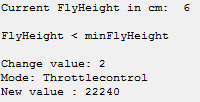
\includegraphics[width=0.4\textwidth]{Billeder/Test/skift_hoejde.png}
\caption{Tilpasning af flyvehøjde}
\label{fig:skift_hoejde}
\end{figure}

\begin{figure}[H]
\centering
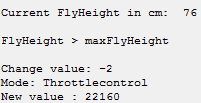
\includegraphics[width=0.4\textwidth]{Billeder/Test/skift_hoejde2.png}
\caption{Tilpasning af flyvehøjde}
\label{fig:skift_hoejde2}
\end{figure}

Selvom flyvehøjden er indenfor intervallet, vil der stadig reguleres. Dette gøres for at holde dronen stabil og indenfor intervallet. Selve reguleringen foregår i mindre steps end hvis flyvehøjden var udenfor intervallet.
Figur \ref{fig:interval_skift} viser hvad den aktuelle flyvehøjde er og hvor meget den er skiftet siden sidste måling.

\begin{figure}[H]
\centering
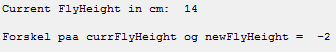
\includegraphics[width=0.6\textwidth]{Billeder/Test/hoejdei_interval_skift.png}
\caption{Interval højde skift}
\label{fig:interval_skift}
\end{figure}